\chapter{Paths, Areas and Groups}\label{chap:chap4}
\special{pdf: out 1 << /Title (\thechapter. Paths, Areas and Groups) /Dest [ @thispage /FitH @ypos ] >>}

SteamCAD2 introduces new types of objects - paths, areas and groups. The path consists of
two or more connected line segments. The aim of path is to produce better layout of dash patterns.
The area consists of one or more closed paths. It can be filled with a solid color. Translucency
is also supported. A group is simply a collection of independent objects, for better manipulation
such as copying, moving etc.

\section{Create path}\label{sec:createpath}
\special{pdf: out 2 << /Title (\thesection. Create path) /Dest [ @thispage /FitH @ypos ] >>}

Attempts to create path from selected segments. It can create one or more paths depending on
the segments connectivity. A path can also be among the selected segments, and if possible,
it will be extended by other segments.

\section{Create area}\label{sec:createarea}
\special{pdf: out 2 << /Title (\thesection. Create area) /Dest [ @thispage /FitH @ypos ] >>}

Attempts to create area from selected paths or segments. First it attempts to create paths,
then area object. The winding rule is alternative, the paths should not cross. For selfcrossing
paths or crossing paths, the result is unpredicable. The usage of paths and areas are demonstrated
in the figure~\ref{fig:csd_mark}.

\begin{figure}[h]
\begin{center}
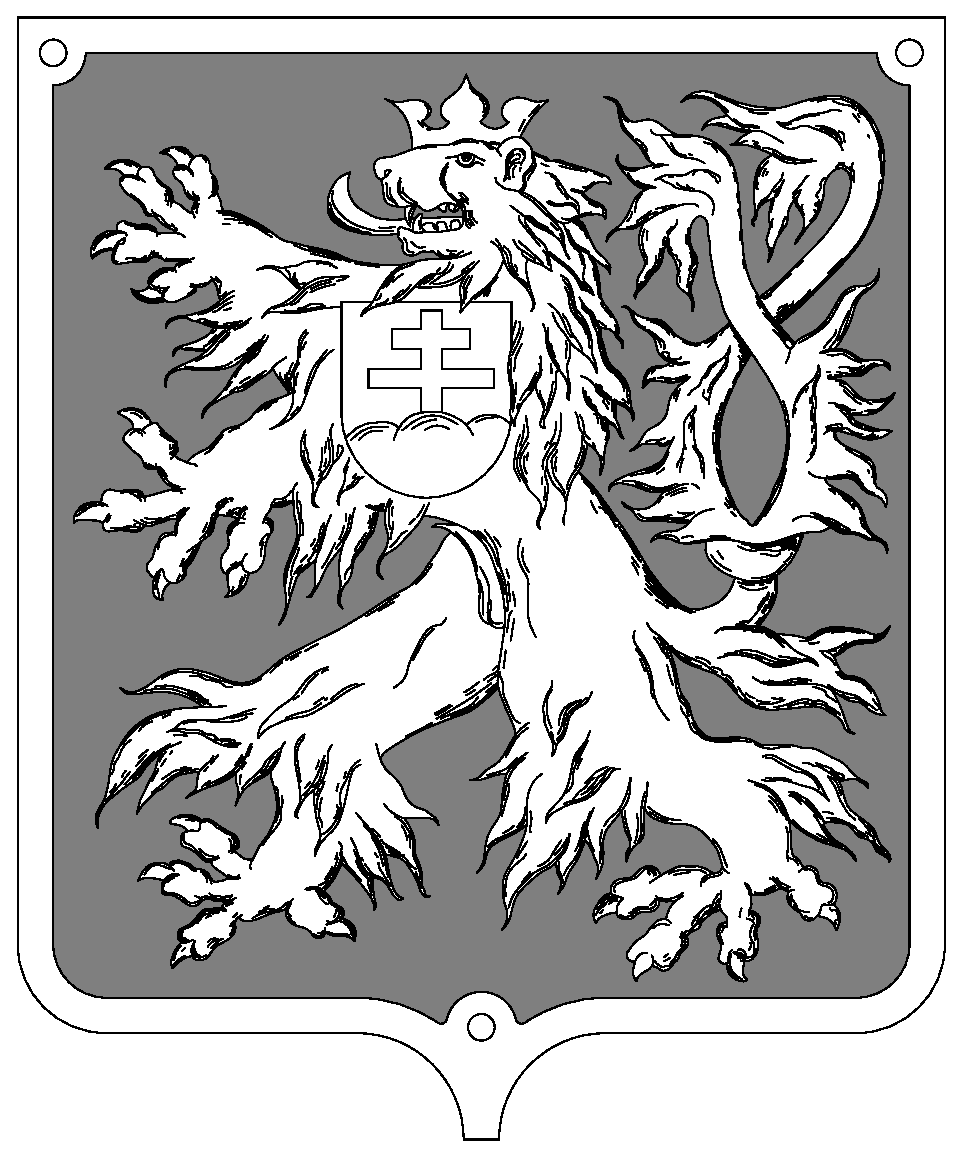
\includegraphics[scale=0.3]{Images/csd_mark.eps}
\end{center}
\caption{The emblem of Czechoslovak railways used from 1920 to 1939}
\label{fig:csd_mark}
\end{figure}

\section{Break apart}\label{sec:breakapart}
\special{pdf: out 2 << /Title (\thesection. Break apart) /Dest [ @thispage /FitH @ypos ] >>}

Breaks a path or area. In case of a path, it is decomposed to the original segments. An area
is decomposed to the paths which defines it.

\section{Release frontiers}\label{sec:releasefront}
\special{pdf: out 2 << /Title (\thesection. Release frontiers) /Dest [ @thispage /FitH @ypos ] >>}

If you create a path sequentially, it may happen that the next segment is not properly aligned
with the last segment of a path. Since it is impossible to edit path, braking the whole path
might result in a lots of lost work. This command can be used to release the first and last
segment of a path, which allows to edit the last segment to properly align with the next
segment to be added to the path.

\section{Group}\label{sec:group}
\special{pdf: out 2 << /Title (\thesection. Group) /Dest [ @thispage /FitH @ypos ] >>}

Groups selected objects into a single group object. Groups can be nested.

\section{Ungroup}\label{sec:ungroup}
\special{pdf: out 2 << /Title (\thesection. Ungroup) /Dest [ @thispage /FitH @ypos ] >>}

Ungroup a group. If the group contained other groups, the subgroups would not be affected.

\section{Move up, down, top and bottom}\label{sec:moveupdown}
\special{pdf: out 2 << /Title (\thesection. Move up, down, top and bottom) /Dest [ @thispage /FitH @ypos ] >>}

With presence of groups and areas, the drawing orger of the objects becomes important.
These commands can be used to move objects in the drawing list, thus makes them
appearing above or under other objects.
